%----------------------------------------------------------------
%
%  File    :  survey-animation.tex
%
%  Author  :  Fernando Pulido Ruiz, TU Graz, Austria
% 
%  Created :  01 Dec 2016
% 
%  Changed :  X Dec 2016
% 
%----------------------------------------------------------------


\chapter{Animation}

\label{chap:Animation}

{\em"Animation is defined as changing some property over time. On the other hand, motion is the act of moving or the process of being moved. . . .  To put it more simply, all motion is animation, but not all animation is motion."}\citep{head2016designing}

\TODO{\section{sections by F.P.R.}} % (fold)
\label{sec:anime_sthg}


\begin{figure}[tp]
\centering
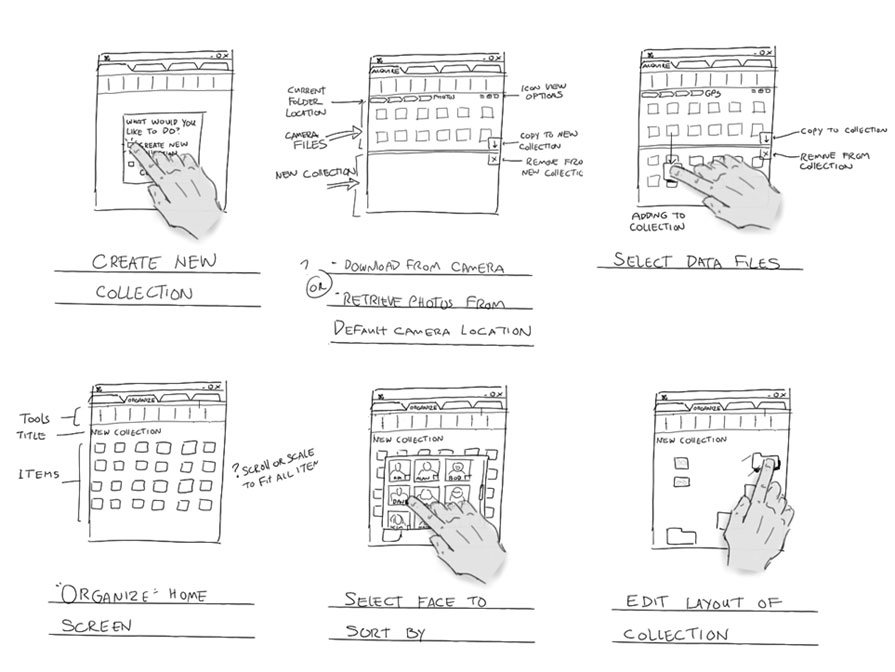
\includegraphics[keepaspectratio,width=\hsize,height=\halfh]
{images/storyboard.jpeg}

\caption[Storyboard Sketching]{
Example of storyboard sketching for drag and drop animation \citep{microsoftStoryboard}.
\imgcredit{Used with permission from Microsoft - Microsoft Copyrighted Content Guidelines}
}
\label{fig:storyboard}
\end{figure}

% section CSS_Examples (end)